\chapter{Bevezetés}

\thispagestyle{fancy}
\pagestyle{fancy}
\nomenclature{$AI$}{Artificial Intelligence (Mesterséges Intelligencia)}

A szöveg normál stílusú: Times New Roman, 12 pt, 1.5-ös sortávolságú, sorkizárt. A változók szövegben dőlt betűvel szerepeljenek. Az új bekezdés első sora behúzással új sorban, nem előzi meg üres sorköz (sablon alapértelmezett stílusa).\par
Címek értelemszerűen számozva, Heading 1: 14 pt, Times New Roman/Computer Modern, félkövér, további Heading: 12 pt, félkövér, Times New Roman/Computer Modern, minden cím előtt és után a dokumentum alapértelmezett stílusában vannak beállítva a sorközök, cím utáni első bekezdés stílusa.\par
A formátum beállítását szerkeszteni NEM kell, a dokumentum alapértelmezései tartalmazzák azokat.\\
Általános szabályok:
\begin{itemize}
    \item minden műveleti jelet (számtani, halmazelméleti stb.) megelőz és követ egy-egy szóköz,
    \item minden írásjelet (pont, vessző, kérdőjel, stb,) követ egy szóköz,
    \item a zárójelek: normál (nem dőlt).
\end{itemize}
\textbf{Nyelvi ajánlás:} magyar ill. angol nyelv szempontjából a Magyar Helyesírási Szabályzat, ill. a megfelelő – brit, amerikai stb. – angol nyelvi szabályzat.\\
\textbf{Terjedelem:} a tartalmi rész legalább 40 oldal, de legfeljebb 60 oldal.\\
\textbf{Margók:} normál (felső, alsó, bal és jobb oldali margók is egyaránt 2,54 cm-esek, a kötésmargó 1 cm.)\\
\textbf{Oldalszámozás:} középre alulra. Fejléc tartalma fejezetenként a fejezetcímek középre rendezve.\par

\section{Alfejezet}

A tartalmi részt a témavezető és a hallgató közösen határozzák meg, mely a jelölt idézetek nélkül legalább a dolgozat 2/3-a, legalább 40 oldal.\par
Néhány mondatnál hosszabb szövegszerű idézeteket az érdemi részbe berakni NEM szabad. Hosszabb idézetet a Mellékletben kell elhelyezni, a forrás megjelölés minden esetben kötelező.

\subsection{Al-alfejezet}
Ábrák, képletek középre rendezve, feliratozva és számozva kerüljenek a dolgozatba. A felirat az ábra alatt foglal helyet.\\
Ábra elhelyezése a laTex fájlban a következő kódrészlettel történik:\\
\begin{figure}[H]
    \centering %középre igazítja a képet
    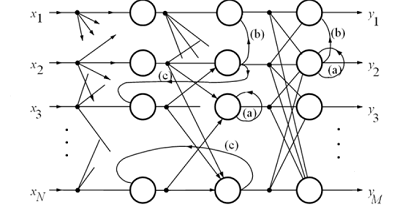
\includegraphics{img/minta1.png} %a képfájl neve, elérési útvonallal, ha külön mappában helyezzük el
    \caption{Képaláírás szövege \cite{detection16}} % a \cite{detection03} a hivatkozott forrás megjelölésére szolgál
    \label{fig:fig_minta1} %a kép label -ét használjuk a folyó szövegben a képre való hivatkozáskor. Ennek segítségével a laTex a sorszámozás változását, követését automatikusan elvégzi
\end{figure}
Az ábrákra a dolgozat szövegében hivatkozni kell, magyarázattal kell ellátni őket, például a \ref{fig:fig_minta1} ábra egy minta ábra ebben a sablonban, útmutatóban.

\subsubsection{Táblázatok elhelyezése}
A táblázatok középre rendezve, feliratozva és számozva kerüljenek a dolgozatba. A táblázat felirata a táblázat felett helyezkedik el.\par
Táblázaton belül a szöveg függőlegesen középre igazítva. Az adatok vízszintes igazítását az adattartalom határozza meg (decimális értékek esetén javasolt a decimális igazítás).\par
A dolgozat szövegésben pl. ilyen módon lehet hivatkozni a mybib.bib fájlban összegyűjtött szakirodalmakra, forrásokra \cite{detection01, detection02}.

\begin{table}[!h]
\caption{Minta táblázat}
\label{tab:minta_tablazat} %ezzel a label-el kell hivatkozni a táblázatra a folyó szövegben, a képekhez hasonló módon
\resizebox{\linewidth}{!}{%
\begin{tabular}{ccccc} %annyi karakter, ahany oszlop van a tablazatban
\hline %vizszintes vonal
\multicolumn{1}{l}{\textbf{Szöveg/Szöveg2}} &
  \textbf{\begin{tabular}[c]{@{}c@{}}cella fejléc 1. sor\\  cella fejléc 2. sor\end{tabular}} &
  \textbf{\begin{tabular}[c]{@{}c@{}}2. cella fejléc első sor \\2. cella fejléc 2. sor\end{tabular}} &
  \textbf{\begin{tabular}[c]{@{}c@{}}3. cella fejléc első sor \\3. cella fejléc 2. sor\end{tabular}} &
  \textbf{\begin{tabular}[c]{@{}c@{}}4. cella fejléc első sor \\4. cella fejléc 2. sor\end{tabular}} \\ \hline
\textbf{1. oszlop 1. sor fejléc} & Adat1 & Adat2 & Adat3 & Adat4 \\
\textbf{1. oszlop 2. sor fejléc} & Adat5 & Adat6 & Adat7 & Adat8  \\
\textbf{secondary grade, specialized} & Adat9 & Adat10 & Adat11 & Adat12 \\
\textbf{1. oszlop 3. sor fejléc} & Adat13 & Adat14 & Adat15 & Adat16 \\
\hline
\multicolumn{1}{|c|}{\textbf{Number of data}} & \multicolumn{1}{c|}{Adat17} & \multicolumn{1}{c|}{Adat18} & \multicolumn{1}{c|}{Adat19} & \multicolumn{1}{c|}{Adat20} \\
\hline
Percent(\%) of 46 & 33\% & Adat21\% & Adat22\% & Adat23\%
\end{tabular}%
}
\end{table}
A szövegben a táblázatra is kell utalni, el kell látni magyarázattal, például a \ref{tab:minta_tablazat} táblázatra így hivatkozunk. 